\label{chap:background}

In this Chapter, we discuss relevant background information toward the goal of implementing a packetized display protocol (PDP) architecture for IRLED projector systems. First, we give an overview of what constitutes an IRLED system. Following this, we discuss in general how common display protocols work to send pixel data to a display system (e.g. a television). Finally, we discuss how these protocols are utilized within an IRLED system including discussion of example scenarios.

\section{IRLED Projector Systems}

\section{Classical Display Protocols}
    \label{sec:classical_display_protocols}

    Classical display protocols such as (DVI\cite{DDWG1999}, HDMI\cite{HDMIForum2018}, and DisplayPort\cite{VESA2016} are commonly used for driving consumer electronic devices. These generally provide a standardized feature-set that is rooted in classical analog video specifications (e.g. VGA, Composite)\cite{NIAnalog} which utilize scan lines\cite{Neal1998}. Scan lines are used to provide video timing information in order to synchronize a display to a given refresh-rate. Each scan line consist of an active video region followed by a horizontal blanking period. After all active video scan lines are displayed, a vertical synchronization region is used to indicate the end of a frame.

    \begin{figure}
        \centering
        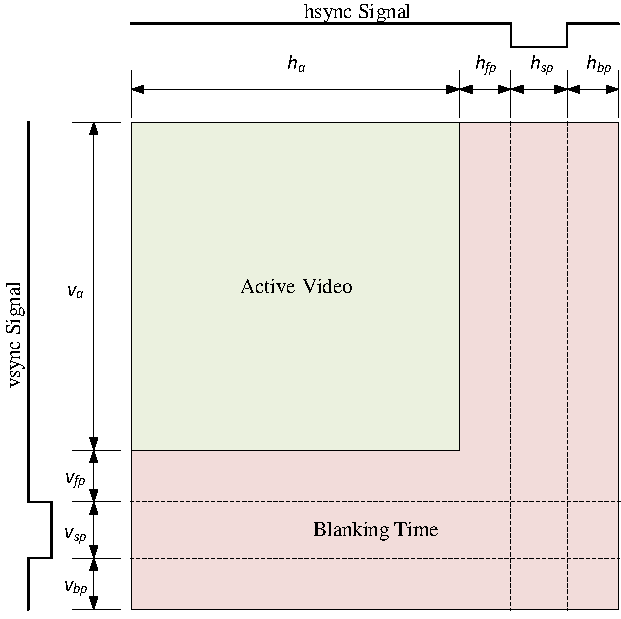
\includegraphics[width=1.0\textwidth]{fig/display_timing_overview.pdf}
        \caption{Display Protocol Timing Overview}
        \label{fig:display_protocol_timing_overview}
    \end{figure}

    \begin{figure}
        \centering
        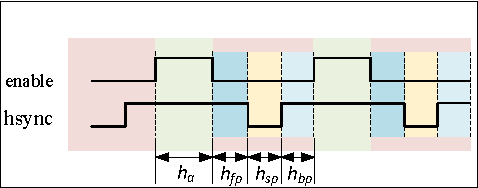
\includegraphics[width=1.0\textwidth]{fig/display_timing_line_cross.pdf}
        \caption{Display Protocol Horizontal Signal Cross Section Timing}
        \label{fig:display_protocol_line_cross}
    \end{figure}

    %FIXME add crosssectional blowout chart

    An overview of this is shown in Figure \ref{fig:display_protocol_timing_overview}. The region shown in green is the pixel data for the active video region of the display. It is of size $H_a\times V_a$ which represents the number of pixels to display, for example, 1920 by 1080 for a HDTV high-definition video mode\cite{MythTVWebsite}. The blanking time regions denote pixel data that is sent but not displayed\footnote{Typically data lines are held low during this period, but somtimes it is used for out-of-band communication to send other information such as audio encoding for example.}. A scan line consist of pixels made up of $h_a$, the horizontal active size; $h_{fp}$, the horizontal front porch before the pulse signal; $h_{sp}$, the horizontal sync pulse; and $h_{bp}$, the horizontal back porch after the sync pulse. The vertical blanking period makes up multiple scanlines and consist of $v_{fp}$, the vertical front porch before the vsync pulse; $v_{sp}$, the vertical sync pulse; $v_{bp}$, the vertical back porch after the vertical sync pulse. In practice, sync pulses are generally active low, meaning that during active display a sync signal is high as shown in the diagram.

    Figure \ref{fig:display_protocol_line_cross} shows a closeup view of signal lines during the active region of display for two scan lines. A data enable signal denoted by $en$ is high during the active region shown in green. Following this, it goes low for a period of time denoted by $h_{fp}+h_{sp}+h_{bp}$. The horizontal sync signal goes low only in the region shown in yellow between the front porch and back porches. This process repeats for all scan lines. Once the last active region pixel is drawn, the enable signal will stop going high during the vertical synchronization period.

    %FIXME: Fix discussion of DP not using fucking backwards compatibility shitty hdmi fucking mode
    %FIXME: Talk about CC in the vertical blanking

    \begin{figure}
        \centering
        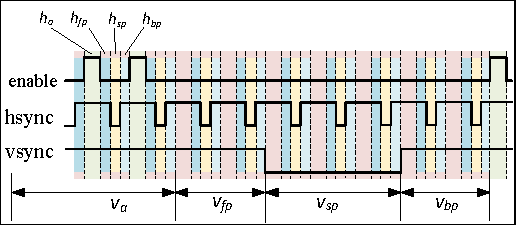
\includegraphics[width=1.0\textwidth]{fig/display_timing_full_cross.pdf}
        \caption{Display Protocol Full Signal Cross Section Timing}
        \label{fig:display_protocol_full_cross}
    \end{figure}

    Figure \ref{fig:display_protocol_full_cross} shows a closeup view of signal lines during the transition into the vertical synchronization period. The region donated by $V_a$ indicates the end of the video active region of the display which occurs toward the end of a frame. After the active video region, all data has been drawn to a display. The region denoted by $v_{fp}+v_{sp}+v_{bp}$ is the vertical blanking or vsync period during which no active video data is sent; therefore, data enable denoted by $en$ is always low during this period. Before the vertical sync pulse period denoted by $v_{sp}$ occurs, a vertical front porch period denoted by $v_{fp}$ occurs. After the vertical sync pulse, a vertical back porch region $v_{bp}$ occurs. Following this the beginning of the next frame occurs as denoted by $v_{a+1}$.
    \begin{figure}
        \centering
        { \Large
            $l_h=h_a+h_{fp}+h_{sp}+h_{bp}$ \vspace{8px} \\
            $l_v=v_a+v_{fp}+v_{sp}+v_{bp}$ \vspace{8px} \\
            $f_f={f_p \over {l_h \cdot l_v}}$ \\
            $p_t={1 \over f_p}$ \vspace{8px} \\
            $f_t={1 \over f_f}$ \vspace{8px}
        }
        \caption{Total Refresh Rate}
        \label{fig:modeline_refresh_rate}
    \end{figure}

    Figure \ref{fig:modeline_refresh_rate} shows the relationship between between the different regions of a display and the frequency or refresh rate. $l_h$ denotes the scan line size of a display, or total horizontal width, which is made up of the horizontal active and horizontal porch region pixels of a display. $l_v$ denotes the total vertical width of a display, which is made up the vertical active and vertical porch region pixels of a display. Each pixel is sent at a rate denoted by $f_p$, the pixel frequency (also called the pixel clock). $f_f$ denotes the frame frequency or framerate of a display. This is simply the pixel frequency over the total number of pixels (video active and porches) of a display. $p_t$ denotes the time period a single pixel takes to send. $f_t$ denotes the time period for an entire frame.

    \begin{figure}
        \centering
        { \normalsize
        \textbf{``1920x1080\_30.00"} {\color{red}79.75}  {\color{blue} 1920 1976 2168 2416}  {\color{darkgreen}1080 1083 1088 1102} {\color{olive}-hsync +vsync}
        %\vspace{-8px}
        }
        \caption{VESA CVT Generated Modeline}
        \label{fig:modeline_example}
    \end{figure}

    %FIXME: example modeline
    To illustrate, let us look at the display modeline generated using the VESA Coordinated Video Timing (CVT) standard shown in Figure \ref{fig:modeline_example}. This modeline operates a total frame frequency of $30.0hz$. The pixel clock 79.75, denoted in red, is specified in megahertz. The horizontal pixels, denoted in blue; are horizontal active, horizontal front porch, horizontal sync pulse, and horizontal back porch respectively. The vertical pixels (measured in lines), are denoted in green; are vertical active, vertical front porch, vertical sync pulse, and horizontal back porch respectively. The sync pulse polarities, denoted in yellow; indicate whether a given sync pulse is active low or active high. A minus symbol indicates active low and a plus symbol indicates active high. If we put these numbers into the formulas shown in Figure \ref{fig:modeline_refresh_rate} we yield the results shown in Figure \ref{blah}.

    %FIXME: finish this chart
    \begin{figure}
        \centering
        { \Large
            $l_h=1920+1976+2168+2416$ \vspace{8px} \\
            $l_v=1080+1083+1088+1102$ \vspace{8px} \\
            $f_p=79.75e6$ \vspace{8px} \\
            $f_f=30.0={f_p \over {l_s \cdot l_c}}$ \\
            $p_t={1 \over f_p}$ \vspace{8px} \\
            $f_t={1 \over f_f}$ \vspace{8px}
        }
        \caption{Computed Refresh Rate for a 30hz CVT Modeline}
        \label{fig:modeline_refresh_rate_plug}
    \end{figure}

\section{Display Protocols within an IRLED Project System}
